%============================================================================
%  WODLIE ENGINE — Pitch Deck / Propuesta de Negocio
%  Motor: pdfLaTeX  ·  Clase: beamer 16:9
%  Compilar:  latexmk -pdf wodlie-engine-pitch.tex
%             (o: pdflatex dos veces)
%============================================================================
\documentclass[aspectratio=169,10pt]{beamer}

%----------------------------------------------------------------------------
%  Fuentes (Fira Sans — moderna, geométrica, legible en pantalla)
%----------------------------------------------------------------------------
\usepackage[T1]{fontenc}
\usepackage[utf8]{inputenc}
\usepackage[sfdefault]{FiraSans}
\usepackage[scaled=0.85]{FiraMono}
\renewcommand*\familydefault{\sfdefault}
\usepackage{microtype}

%----------------------------------------------------------------------------
%  Gráficos y cajas
%----------------------------------------------------------------------------
\usepackage{tikz}
\usetikzlibrary{positioning,arrows.meta,shapes.geometric,calc,shadows.blur}
\usepackage[most]{tcolorbox}
\usepackage{fontawesome5}
\usepackage{array}
\usepackage{ragged2e}

%----------------------------------------------------------------------------
%  Paleta de marca Wodlie Engine
%----------------------------------------------------------------------------
\definecolor{wink}{HTML}{4F46E5}   % indigo — primario
\definecolor{wink2}{HTML}{6366F1}  % indigo claro
\definecolor{wcyan}{HTML}{06B6D4}  % cian — acento
\definecolor{wdark}{HTML}{0B1220}  % fondo oscuro
\definecolor{wslate}{HTML}{334155} % texto
\definecolor{wgray}{HTML}{64748B}  % texto secundario
\definecolor{wlight}{HTML}{EEF2FF} % fondo suave indigo
\definecolor{wline}{HTML}{E2E8F0}  % bordes
\definecolor{wmint}{HTML}{10B981}  % verde
\definecolor{wamber}{HTML}{F59E0B} % ámbar
\definecolor{wrose}{HTML}{F43F5E}  % rosa

%----------------------------------------------------------------------------
%  Tema Beamer minimalista y plano (sin barras de navegación)
%----------------------------------------------------------------------------
\usetheme{default}
\usefonttheme{professionalfonts}
\setbeamertemplate{navigation symbols}{}
\setbeamertemplate{itemize items}{\color{wink}\scriptsize$\blacktriangleright$}
\setbeamertemplate{itemize subitem}{\color{wcyan}\scriptsize$\blacktriangleright$}
\setbeamercolor{normal text}{fg=wslate}
\setbeamercolor{structure}{fg=wink}
\setbeamercolor{frametitle}{fg=wdark,bg=white}
\setbeamercolor{background canvas}{bg=white}
\setbeamerfont{frametitle}{series=\bfseries,size=\Large}
\setbeamerfont{title}{series=\bfseries}

% --- Título de frame con filete de acento -------------------------------
\setbeamertemplate{frametitle}{%
  \vspace*{0.55em}%
  \hspace*{0.2em}{\color{wink}\rule[-0.15em]{3pt}{1.15em}}\hspace{0.5em}%
  {\usebeamerfont{frametitle}\usebeamercolor[fg]{frametitle}\insertframetitle}%
  \par\vspace*{-0.2em}%
}

% --- Pie de página: marca + número --------------------------------------
\setbeamertemplate{footline}{%
  \hbox{\begin{beamercolorbox}[wd=\paperwidth,ht=2.4ex,dp=1.2ex,leftskip=1.2em,rightskip=1.2em]{}%
    {\color{wgray}\footnotesize\bfseries wodlie\,{\color{wink}engine}}%
    \hfill{\color{wgray}\footnotesize Propuesta de negocio · Confidencial}%
    \hfill{\color{wgray}\footnotesize\insertframenumber}%
  \end{beamercolorbox}}%
}

%----------------------------------------------------------------------------
%  Estilos de tarjetas (tcolorbox)
%----------------------------------------------------------------------------
\tcbset{
  wcard/.style={
    enhanced, colback=white, colframe=wline, boxrule=0.8pt, arc=6pt,
    drop fuzzy shadow=black!12, left=8pt, right=8pt, top=7pt, bottom=7pt,
    fontupper=\small
  },
  wtitle/.style={
    enhanced, colback=white, colframe=white, arc=6pt,
    drop fuzzy shadow=black!12, boxrule=0pt,
    borderline west={3pt}{0pt}{#1},
    left=10pt, right=8pt, top=4.5pt, bottom=4.5pt, fontupper=\small
  },
  wfill/.style={
    enhanced, colback=#1!12, colframe=#1, boxrule=0.8pt, arc=6pt,
    left=8pt, right=8pt, top=7pt, bottom=7pt, fontupper=\small
  },
}

% Tarjeta con encabezado de color
\newtcolorbox{hcard}[2][wink]{%
  enhanced, colback=white, colframe=#1, boxrule=1pt, arc=6pt,
  drop fuzzy shadow=black!12,
  coltitle=white, colbacktitle=#1, fonttitle=\bfseries\small,
  title=#2, left=8pt, right=8pt, top=6pt, bottom=7pt, fontupper=\small,
  attach boxed title to top left={xshift=8pt,yshift=-3pt},
  boxed title style={arc=3pt,boxrule=0pt}
}

%----------------------------------------------------------------------------
%  Comandos de ayuda
%----------------------------------------------------------------------------
% Diapositiva divisora de sección (fondo oscuro)
\newcommand{\divider}[3]{% #1 número  #2 título  #3 subtítulo
{\setbeamercolor{background canvas}{bg=wdark}%
\begin{frame}[plain]
  \begin{tikzpicture}[remember picture,overlay]
    \fill[wink] (current page.north west) rectangle ([xshift=6pt]current page.south west);
    \node[anchor=west,text=wcyan] at ([xshift=1.4cm,yshift=1.7cm]current page.west)
      {\fontsize{54}{54}\selectfont\bfseries #1};
    \node[anchor=west,text=white,align=left] at ([xshift=1.4cm,yshift=0.1cm]current page.west)
      {\fontsize{26}{30}\selectfont\bfseries #2};
    \node[anchor=west,text=wgray,align=left,text width=9cm] at ([xshift=1.42cm,yshift=-1.35cm]current page.west)
      {\normalsize #3};
    \node[anchor=south east,text=wgray] at ([xshift=-0.8cm,yshift=0.6cm]current page.south east)
      {\footnotesize wodlie\,{\color{wink2}engine}};
  \end{tikzpicture}
\end{frame}}
}

% Píldora / etiqueta
\newcommand{\pill}[2][wink]{\tikz[baseline=(x.base)]\node[fill=#1!15,text=#1,rounded corners=3pt,inner xsep=5pt,inner ysep=2pt,font=\footnotesize\bfseries](x){#2};}

% KPI grande
\newcommand{\kpi}[3][wink]{\begin{tcolorbox}[enhanced,colback=white,colframe=wline,boxrule=0.8pt,arc=6pt,drop fuzzy shadow=black!12,halign=center,left=2pt,right=2pt,top=4pt,bottom=4pt]{\color{#1}\fontsize{15}{15}\selectfont\bfseries #2}\\[1pt]{\color{wgray}\scriptsize #3}\end{tcolorbox}}

\newcommand{\chk}{{\color{wmint}\faCheckCircle}~}
\newcommand{\arw}{{\color{wcyan}\faArrowRight}~}

% Ajusta cualquier contenido (p.ej. un tikzpicture) al ancho de línea:
% solo reduce si es más ancho que \linewidth; nunca lo agranda.
\newcommand{\fitwidth}[1]{\resizebox{\ifdim\width>\linewidth\linewidth\else\width\fi}{!}{#1}}

%============================================================================
\begin{document}

%---------------------------------------------------------------- PORTADA ---
{\setbeamercolor{background canvas}{bg=wdark}
\begin{frame}[plain]
  
\begin{tikzpicture}[remember picture,overlay]
    % acentos geométricos de fondo
    \fill[wink,opacity=0.18] ([xshift=-3cm,yshift=3cm]current page.north east) circle (5cm);
    \fill[wcyan,opacity=0.12] ([xshift=1cm,yshift=-1cm]current page.south west) circle (4cm);
    \draw[wink,line width=6pt] ([xshift=1.4cm,yshift=1.9cm]current page.west) -- ++(0,-3.9cm);

    \node[anchor=west,align=left] at ([xshift=1.9cm,yshift=1.75cm]current page.west)
      {\color{white}\fontsize{40}{44}\selectfont\bfseries wodlie\,{\color{wcyan}engine}};
    \node[anchor=north west,align=left,text width=11cm] at ([xshift=1.92cm,yshift=0.75cm]current page.west)
      {\color{wgray}\fontsize{15}{20}\selectfont Ingeniería de software para PyMEs, del \textit{onboarding} al \textit{deploy}, automatizada y potenciada con IA.};

    \node[anchor=north west] at ([xshift=1.92cm,yshift=-1.35cm]current page.west)
      {\pill[wcyan]{Propuesta de negocio}\;\pill[wink2]{Modelo suscripción}\;\pill[wmint]{Colombia · Argentina}};

    \node[anchor=south west,text=wgray] at ([xshift=1.92cm,yshift=0.7cm]current page.south west)
      {\footnotesize S4WLAND · \today\ · Documento confidencial};
  \end{tikzpicture}
\end{frame}}

%----------------------------------------------------------------- AGENDA ---
\begin{frame}{Agenda}
  \begin{columns}[T]
    \begin{column}{0.5\textwidth}
      \begin{tcolorbox}[wtitle=wink]
        \textbf{01 · El problema}\\ Por qué las PyMEs sufren con el software
      \end{tcolorbox}\vspace{2pt}
      \begin{tcolorbox}[wtitle=wcyan]
        \textbf{02 · La solución}\\ Wodlie Engine y su arquitectura
      \end{tcolorbox}\vspace{2pt}
      \begin{tcolorbox}[wtitle=wmint]
        \textbf{03 · Flujo automatizado}\\ De \textit{onboarding} a \textit{deploy} + oficina virtual con IA
      \end{tcolorbox}\vspace{2pt}
      \begin{tcolorbox}[wtitle=wamber]
        \textbf{04 · Modelo de negocio}\\ Servicios para PyMEs y suscripción mensual
      \end{tcolorbox}
    \end{column}
    \begin{column}{0.5\textwidth}
      \begin{tcolorbox}[wtitle=wrose]
        \textbf{05 · Go-to-market}\\ Adquisición en Colombia y Argentina
      \end{tcolorbox}\vspace{2pt}
      \begin{tcolorbox}[wtitle=wink2]
        \textbf{06 · Equipo}\\ Trabajo con programadores y células
      \end{tcolorbox}\vspace{2pt}
      \begin{tcolorbox}[wtitle=wcyan]
        \textbf{07 · Expansión}\\ Fases de crecimiento regional
      \end{tcolorbox}\vspace{2pt}
      \begin{tcolorbox}[wtitle=wmint]
        \textbf{08 · Primeros pasos}\\ Web, redes, presencia online y \textit{roadmap}
      \end{tcolorbox}
    \end{column}
  \end{columns}
\end{frame}

%============================================================ 01 PROBLEMA ===
\divider{01}{El problema}{Contratar software a medida es caro, lento y opaco. La PyME latinoamericana queda atrapada entre plantillas rígidas y agencias inalcanzables.}

\begin{frame}{Las PyMEs no pueden acceder a ingeniería seria}
  \vspace{0.2em}
  \begin{columns}[T]
    \begin{column}{0.5\textwidth}
      \begin{hcard}[wrose]{\faMoneyBillWave~~Costos de entrada altos}
        Un MVP a medida arranca en \textbf{USD 3.000–7.000} y un sistema completo supera los \textbf{USD 25.000–80.000}. Fuera de alcance para la mayoría de PyMEs.
      \end{hcard}\vspace{6pt}
      \begin{hcard}[wamber]{\faClock~~Tiempos y fricción}
        Cotizaciones que tardan semanas, pagos por hitos (30/30/40) y procesos de \textit{onboarding} manuales que retrasan el arranque.
      \end{hcard}
    \end{column}
    \begin{column}{0.5\textwidth}
      \begin{hcard}[wink]{\faEyeSlash~~Opacidad y riesgo}
        El cliente no sabe qué paga ni cómo avanza. Sin visibilidad del alcance, el precio ni el estado del proyecto.
      \end{hcard}\vspace{6pt}
      \begin{hcard}[wslate]{\faTools~~Mantenimiento abandonado}
        El mantenimiento cuesta \textbf{15–20\% anual} pero suele venderse mal: entregan y desaparecen. El software se degrada.
      \end{hcard}
    \end{column}
  \end{columns}
  \vspace{6pt}
  \begin{center}\small\color{wgray}
    \faLightbulb~ \textbf{Oportunidad:} para ~70\% de las PyMEs la mejor opción es \emph{producto estandarizado + integraciones}, no empezar de cero cada vez.
  \end{center}
\end{frame}

%============================================================ 02 SOLUCIÓN ===
\divider{02}{La solución}{Wodlie Engine convierte cada proyecto en un proceso repetible: un motor que estandariza arquitectura, documentación y entrega para producir software serio a costo marginal.}

\begin{frame}{Qué es Wodlie Engine}
  \vspace{0.2em}
  \begin{columns}[T]
    \begin{column}{0.56\textwidth}
      \begin{tcolorbox}[wfill=wink]
        \textbf{\faCogs~~Un motor, no una agencia.}\\[3pt]
        CLI (\texttt{@s4wland/wodlie-engine}) que \textbf{genera, gestiona y entrega} proyectos con una arquitectura de 4 capas — para \emph{cualquier} tecnología.
      \end{tcolorbox}
      \vspace{6pt}
      \small
      \chk Estandariza estructura, reglas y documentación\\[3pt]
      \chk \textit{Onboarding} → desarrollo → \textit{deploy} como un pipeline\\[3pt]
      \chk Calidad garantizada por plantilla (32 mandamientos técnicos)\\[3pt]
      \chk Cada cliente = proyecto reproducible y auditable
    \end{column}
    \begin{column}{0.44\textwidth}
      \begin{hcard}[wcyan]{Arquitectura de 4 capas}
        \small
        \textbf{\color{wink}AGENTS.md} · maestro raíz\\[4pt]
        \textbf{\color{wamber}.business} · épicas, historias, reportes\\[4pt]
        \textbf{\color{wmint}.infra} · Docker, CI/CD, \textit{deploy}\\[4pt]
        \textbf{\color{wcyan}.dev} · stack, código, guidelines\\[4pt]
        \textbf{\color{wgray}.core} · router y reglas universales
      \end{hcard}
    \end{column}
  \end{columns}
\end{frame}

%======================================================= 03 FLUJO / PIPELINE ===
\divider{03}{El flujo automatizado}{Del primer contacto al deploy, sin fricción: cada etapa disparada por el motor y asistida con IA. Menos trabajo manual, más proyectos en paralelo.}

\begin{frame}{Pipeline: de \textit{onboarding} a \textit{deploy}}
  \vspace{0.1em}
  \begin{center}
  \fitwidth{%
  \begin{tikzpicture}[
      node distance=3.5mm,
      stage/.style={draw=wink,fill=wink!8,rounded corners=5pt,line width=0.8pt,
        text width=2.05cm,minimum height=1.35cm,align=center,font=\scriptsize\bfseries,inner sep=3pt},
      ai/.style={draw=wcyan,fill=wcyan!10},
      auto/.style={draw=wmint,fill=wmint!10},
      arr/.style={-{Stealth[length=2mm]},wgray,line width=1pt}
    ]
    \node[stage,ai] (a) {\faComments\\ Onboarding\\ web};
    \node[stage,ai,right=of a] (b) {\faListUl\\ Discovery\\ guiado};
    \node[stage,ai,right=of b] (c) {\faRobot\\ Cotización\\ IA};
    \node[stage,auto,right=of c] (d) {\faMagic\\ Bootstrap\\ del motor};
    \node[stage,right=of d] (e) {\faCode\\ Desarrollo\\ por células};
    \node[stage,auto,right=of e] (f) {\faVial\\ QA \& CI};
    \node[stage,auto,right=of f] (g) {\faRocket\\ Deploy};
    \foreach \x/\y in {a/b,b/c,c/d,d/e,e/f,f/g}{\draw[arr] (\x) -- (\y);}
    \node[below=1.1cm of d,text=wgray,font=\scriptsize,align=center,text width=12cm]
      {Soporte y evolución continua bajo suscripción $\circlearrowleft$};
    \draw[arr,wmint,dashed] (g.south) |- ([yshift=-0.75cm]d.south) -| (e.south);
  \end{tikzpicture}}
  \end{center}
  \vspace{2pt}
  \begin{columns}[T]
    \begin{column}{0.33\textwidth}
      \small\pill[wcyan]{IA}\; \textbf{Captura \& cotiza}\\[3pt]
      {\color{wgray}\footnotesize Onboarding, discovery y precio estimado sin intervención humana inicial.}
    \end{column}
    \begin{column}{0.33\textwidth}
      \small\pill[wmint]{Auto}\; \textbf{Genera \& despliega}\\[3pt]
      {\color{wgray}\footnotesize Bootstrap, QA, CI/CD y deploy los ejecuta el motor con plantillas.}
    \end{column}
    \begin{column}{0.33\textwidth}
      \small\pill[wink]{Humano}\; \textbf{Diseña \& decide}\\[3pt]
      {\color{wgray}\footnotesize El equipo se concentra en producto y decisiones, no en repetir setup.}
    \end{column}
  \end{columns}
\end{frame}

\begin{frame}{Automatización etapa por etapa}
  \vspace{0.2em}
  \renewcommand{\arraystretch}{1.35}
  \small
  \begin{tcolorbox}[enhanced,colback=white,colframe=wline,boxrule=0.8pt,arc=6pt,drop fuzzy shadow=black!10,left=6pt,right=6pt,top=4pt,bottom=4pt]
  \begin{tabular}{@{}p{2.7cm}p{4.7cm}p{4.9cm}@{}}
    \textbf{\color{wink}Etapa} & \textbf{\color{wink}Hoy (manual)} & \textbf{\color{wink}Con Wodlie Engine} \\[2pt]
    \hline
    Onboarding & Reuniones, correos, formularios sueltos & Portal web con formulario guiado \\
    Discovery & Entrevistas largas, notas dispersas & Cuestionario dinámico por tipo de proyecto \\
    Cotización & Días de estimación humana & \pill[wcyan]{IA} precio estimado en minutos \\
    Bootstrap & Setup repetitivo por proyecto & \pill[wmint]{Auto} \texttt{engine init} genera las 4 capas \\
    Desarrollo & Reglas ad-hoc, calidad variable & Guidelines §1–§32 embebidos \\
    Deploy & Configuración manual frágil & \pill[wmint]{Auto} \texttt{deliver} + CI/CD por plantilla \\
  \end{tabular}
  \end{tcolorbox}
  \vspace{2pt}
  \begin{center}\footnotesize\color{wgray}
    \faBolt~ Resultado: menor costo por proyecto $\Rightarrow$ precios accesibles para PyMEs y márgenes sanos para nosotros.
  \end{center}
\end{frame}

\begin{frame}{Oficina virtual: el cotizador con IA}
  \vspace{0.2em}
  \begin{columns}[T]
    \begin{column}{0.54\textwidth}
      \begin{hcard}[wink]{Flujo self-service del cliente}
        \small
        \textbf{1.}~ Entra al sitio y elige \textbf{tipo de necesidad}\\ \hspace*{1.1em}(landing, e-commerce, app interna, admin…)\\[4pt]
        \textbf{2.}~ Responde un \textbf{cuestionario dinámico}\\ \hspace*{1.1em}(alcance, integraciones, plazos)\\[4pt]
        \textbf{3.}~ La \textbf{IA estima} complejidad y \textbf{precio}\\[4pt]
        \textbf{4.}~ Elige \textbf{plan de suscripción} y contrata\\[4pt]
        \textbf{5.}~ El motor hace \textbf{bootstrap} y arranca
      \end{hcard}
    \end{column}
    \begin{column}{0.46\textwidth}
      \begin{tcolorbox}[wfill=wcyan]
        \textbf{\faRobot~~¿Por qué con IA?}\\[3pt]
        \small Traduce requisitos en lenguaje natural a un \textbf{alcance estructurado} y un \textbf{rango de precio} coherente con nuestras plantillas.
      \end{tcolorbox}
      \vspace{6pt}
      \small
      \chk Precio transparente en minutos, no semanas\\[3pt]
      \chk Califica \textit{leads} automáticamente (\textit{lead scoring})\\[3pt]
      \chk Cliente con expectativas claras desde el día 0\\[3pt]
      \chk Cada cotización alimenta el motor de estimación
    \end{column}
  \end{columns}
\end{frame}

%================================================== 04 MODELO DE NEGOCIO ===
\divider{04}{El modelo de negocio}{Ingeniería como servicio recurrente: la PyME paga una suscripción mensual y recibe software vivo, mantenido y en evolución — no un entregable que se abandona.}

\begin{frame}{Servicios de ingeniería para PyMEs}
  \vspace{0.2em}
  \begin{columns}[T]
    \begin{column}{0.33\textwidth}
      \begin{hcard}[wink]{\faLaptopCode~~Construir}
        \small Landing pages, e-commerce, apps internas, paneles admin y APIs — sobre plantillas probadas.
      \end{hcard}
    \end{column}
    \begin{column}{0.33\textwidth}
      \begin{hcard}[wcyan]{\faSync~~Mantener}
        \small Soporte, correcciones, actualizaciones de seguridad y monitoreo continuo bajo SLA.
      \end{hcard}
    \end{column}
    \begin{column}{0.33\textwidth}
      \begin{hcard}[wmint]{\faChartLine~~Evolucionar}
        \small Nuevas funciones por sprint, integraciones y mejoras guiadas por datos del negocio.
      \end{hcard}
    \end{column}
  \end{columns}
  \vspace{10pt}
  \begin{tcolorbox}[wfill=wink]
    \small \textbf{Posicionamiento:} en vez de vender un proyecto de USD 8.000 que el 90\% de las PyMEs no puede pagar de golpe, vendemos una \textbf{relación mensual} que reparte el costo, garantiza continuidad y genera ingresos recurrentes (MRR).
  \end{tcolorbox}
\end{frame}

\begin{frame}{Modelo de suscripción — planes}
  \vspace{0.1em}
  \begin{columns}[T]
    \begin{column}{0.33\textwidth}
      \begin{tcolorbox}[enhanced,colback=white,colframe=wline,boxrule=1pt,arc=8pt,drop fuzzy shadow=black!12,top=8pt,bottom=8pt]
        \centering{\color{wgray}\bfseries LAUNCH}\\[4pt]
        {\color{wink}\fontsize{24}{24}\selectfont\bfseries \$X}{\color{wgray}\small /mes}\\[6pt]
        \raggedright\footnotesize
        \chk 1 servicio activo\\
        \chk Sitio o app base\\
        \chk Mantenimiento incluido\\
        \chk Soporte por ticket\\
        \chk 1 sprint / mes
      \end{tcolorbox}
    \end{column}
    \begin{column}{0.33\textwidth}
      \begin{tcolorbox}[enhanced,colback=wink!6,colframe=wink,boxrule=1.4pt,arc=8pt,drop fuzzy shadow=black!18,top=8pt,bottom=8pt]
        \centering\pill[wamber]{Más popular}\\[3pt]{\color{wink}\bfseries GROWTH}\\[4pt]
        {\color{wink}\fontsize{24}{24}\selectfont\bfseries \$Y}{\color{wgray}\small /mes}\\[6pt]
        \raggedright\footnotesize
        \chk Hasta 2 servicios\\
        \chk Backend + frontend\\
        \chk Integraciones y pagos\\
        \chk Soporte prioritario\\
        \chk 2 sprints / mes + reportes
      \end{tcolorbox}
    \end{column}
    \begin{column}{0.33\textwidth}
      \begin{tcolorbox}[enhanced,colback=white,colframe=wcyan,boxrule=1pt,arc=8pt,drop fuzzy shadow=black!12,top=8pt,bottom=8pt]
        \centering{\color{wcyan}\bfseries SCALE}\\[4pt]
        {\color{wcyan}\fontsize{24}{24}\selectfont\bfseries \$Z}{\color{wgray}\small /mes}\\[6pt]
        \raggedright\footnotesize
        \chk Suite completa (4 capas)\\
        \chk Célula dedicada\\
        \chk SLA y monitoreo\\
        \chk Roadmap trimestral\\
        \chk Sprints ilimitados*
      \end{tcolorbox}
    \end{column}
  \end{columns}
  \vspace{4pt}
  \begin{center}\footnotesize\color{wgray}
    Precios a calibrar por mercado (COP/ARS/USD). Referencia sector: 64\% de las agencias cobran <\,USD 1.000/mes — hay espacio para valor y margen. \emph{*justo, con cola de trabajo.}
  \end{center}
\end{frame}

\begin{frame}{Ventajas del modelo recurrente}
  \vspace{0.2em}
  \begin{columns}[T]
    \begin{column}{0.5\textwidth}
      \begin{hcard}[wmint]{\faStore~~Para la PyME (cliente)}
        \small
        \chk Sin desembolso inicial grande — \textbf{costo predecible}\\[3pt]
        \chk Software \textbf{siempre mantenido} y seguro\\[3pt]
        \chk Mejora continua, no un entregable congelado\\[3pt]
        \chk Cancelable — \textbf{bajo riesgo} de compromiso\\[3pt]
        \chk Un solo socio técnico, sin contratar equipo
      \end{hcard}
    \end{column}
    \begin{column}{0.5\textwidth}
      \begin{hcard}[wink]{\faChartPie~~Para nosotros (negocio)}
        \small
        \chk \textbf{Ingresos recurrentes} (MRR) predecibles\\[3pt]
        \chk \textbf{LTV alto}, relaciones de largo plazo\\[3pt]
        \chk Motor $\Rightarrow$ costo marginal decreciente\\[3pt]
        \chk Escala sin crecer costos linealmente\\[3pt]
        \chk Valoración de empresa tipo SaaS/servicio
      \end{hcard}
    \end{column}
  \end{columns}
  \vspace{8pt}
  \begin{columns}[T,totalwidth=\textwidth]
    \begin{column}{0.24\textwidth}\kpi[wmint]{\faArrowUp\, MRR}{Ingreso recurrente}\end{column}
    \begin{column}{0.24\textwidth}\kpi[wink]{\faArrowUp\, LTV}{Valor por cliente}\end{column}
    \begin{column}{0.24\textwidth}\kpi[wcyan]{\faArrowDown\, CAC}{Costo de venta}\end{column}
    \begin{column}{0.24\textwidth}\kpi[wamber]{\faArrowDown\, Churn}{Cancelaciones}\end{column}
  \end{columns}
\end{frame}

%================================================== 05 GO-TO-MARKET ===
\divider{05}{Go-to-market}{Empezamos donde el costo-oportunidad es mayor: PyMEs digitalizándose en Colombia y Argentina, dos mercados grandes, hispanohablantes y con talento técnico competitivo.}

\begin{frame}{Colombia y Argentina: dos puntos de entrada}
  \vspace{0.2em}
  \begin{columns}[T]
    \begin{column}{0.5\textwidth}
      \begin{hcard}[wamber]{\faFlag~~Colombia}
        \small
        \chk MVP de mercado: \textbf{USD 4.000–7.000} (COP 16–28M)\\[3pt]
        \chk Landing/sitio: COP 1,5–8M\\[3pt]
        \chk Ecosistema PyME en digitalización acelerada\\[3pt]
        \chk Pagos: PSE, Bold, Wompi, Nequi\\[3pt]
        \chk Hub inicial de operación y captación
      \end{hcard}
    \end{column}
    \begin{column}{0.5\textwidth}
      \begin{hcard}[wcyan]{\faFlag~~Argentina}
        \small
        \chk Devs \textbf{USD 30–55/h}; talento fuerte y accesible\\[3pt]
        \chk MVP desde USD 3.000; intermedio 8–25k\\[3pt]
        \chk Cultura de producto y startups consolidada\\[3pt]
        \chk Pagos: Mercado Pago, transferencias\\[3pt]
        \chk Fuente de talento + base de clientes
      \end{hcard}
    \end{column}
  \end{columns}
  \vspace{6pt}
  \begin{tcolorbox}[wfill=wink]
    \small \textbf{Estrategia:} precio en moneda local + facturación USD para blindar del tipo de cambio. Mismo motor, dos mercados; el talento argentino puede atender clientes de ambos países.
  \end{tcolorbox}
\end{frame}

\begin{frame}{Adquisición de clientes potenciales}
  \vspace{0.1em}
  \begin{center}
  \fitwidth{%
  \begin{tikzpicture}[
      node distance=2mm and 6mm,
      f/.style={rounded corners=4pt,align=center,font=\scriptsize\bfseries,minimum height=0.85cm,text width=3.1cm},
      arr/.style={-{Stealth[length=2mm]},wgray,line width=1pt}]
    \node[f,fill=wcyan!15,text=wcyan] (a) {\faBullhorn\; Atraer\\ contenido · SEO · redes};
    \node[f,fill=wink!15,text=wink,right=of a] (b) {\faFilter\; Captar\\ cotizador IA · lead magnet};
    \node[f,fill=wamber!18,text=wamber!80!black,right=of b] (c) {\faHandshake\; Convertir\\ demo · onboarding web};
    \node[f,fill=wmint!18,text=wmint!70!black,right=of c] (d) {\faHeart\; Retener\\ suscripción · soporte};
    \draw[arr] (a)--(b); \draw[arr] (b)--(c); \draw[arr] (c)--(d);
  \end{tikzpicture}}
  \end{center}
  \vspace{4pt}
  \begin{columns}[T]
    \begin{column}{0.5\textwidth}
      \small\textbf{\color{wink}Canales de entrada}\\[4pt]
      \arw Contenido técnico y casos en LinkedIn / Instagram\\[3pt]
      \arw SEO local (\textit{"software para pymes en …"})\\[3pt]
      \arw Alianzas: cámaras de comercio, gremios, contadores\\[3pt]
      \arw Referidos con incentivo (mes gratis)
    \end{column}
    \begin{column}{0.5\textwidth}
      \small\textbf{\color{wink}Motor de conversión}\\[4pt]
      \arw Cotizador IA como \textit{lead magnet} principal\\[3pt]
      \arw Portafolio y \textit{casos de éxito} verificables\\[3pt]
      \arw Prueba/onboarding sin fricción, 100\% online\\[3pt]
      \arw Nurturing por email/WhatsApp automatizado
    \end{column}
  \end{columns}
\end{frame}

%================================================== 06 EQUIPO ===
\divider{06}{El equipo}{Programadores organizados en células ligeras alrededor del motor: colaboración remota, calidad garantizada por plantilla y pago ligado a la entrega, no a las horas.}

\begin{frame}{Trabajar con programadores y equipos}
  \vspace{0.2em}
  \begin{columns}[T]
    \begin{column}{0.5\textwidth}
      \begin{hcard}[wink]{\faUsers~~Modelo de células}
        \small
        \chk Células pequeñas (2–4 devs) por proyecto/cliente\\[3pt]
        \chk El motor impone estructura $\Rightarrow$ onboarding rápido de nuevos devs\\[3pt]
        \chk Red de \textbf{freelancers} y equipos por demanda\\[3pt]
        \chk Guidelines §1–§32 = calidad homogénea
      \end{hcard}
    \end{column}
    \begin{column}{0.5\textwidth}
      \begin{hcard}[wcyan]{\faBalanceScale~~Cómo colaboran y cobran}
        \small
        \chk Pago por \textbf{entrega/sprint}, no por hora\\[3pt]
        \chk Reparto: base + bono por resultado/cliente retenido\\[3pt]
        \chk Roles: líder de célula, dev, QA, diseño\\[3pt]
        \chk 100\% remoto, async-first (Colombia + Argentina)
      \end{hcard}
    \end{column}
  \end{columns}
  \vspace{8pt}
  \begin{tcolorbox}[wfill=wmint]
    \small \textbf{Ventaja del motor para el equipo:} cualquier dev cae en un proyecto y encuentra la misma arquitectura, reglas y comandos. Menos tiempo entendiendo, más tiempo entregando.
  \end{tcolorbox}
\end{frame}

%================================================== 07 EXPANSIÓN ===
\divider{07}{Plan de expansión}{Crecer por capas, igual que el motor: validar, sistematizar y luego escalar a nuevos mercados y verticales sin perder el margen.}

\begin{frame}{Fases de crecimiento}
  \vspace{0.4em}
  \begin{center}
  \fitwidth{%
  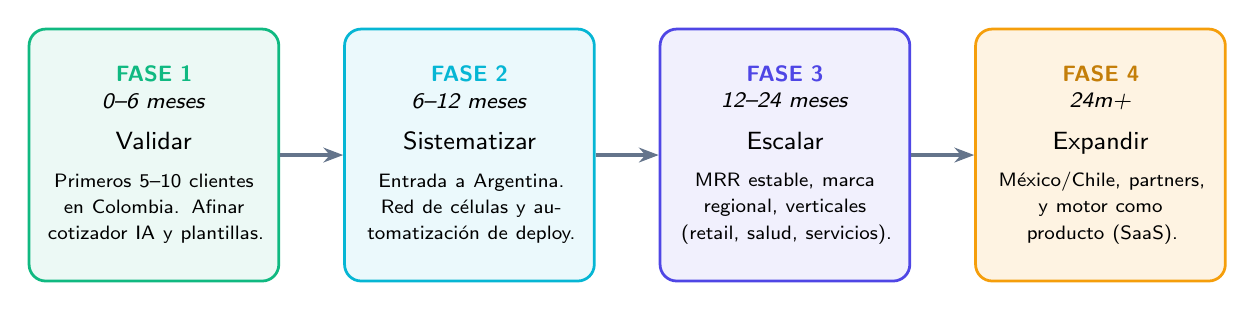
\begin{tikzpicture}[
      node distance=0mm,
      ph/.style={rounded corners=6pt,line width=1pt,text width=2.75cm,minimum height=3.2cm,align=center,inner sep=6pt,font=\footnotesize}]
    \node[ph,draw=wmint,fill=wmint!8] (p1) {\textbf{\color{wmint}FASE 1}\\ \textit{0–6 meses}\\[4pt] \small Validar\\[4pt] \scriptsize Primeros 5–10 clientes en Colombia. Afinar cotizador IA y plantillas.};
    \node[ph,draw=wcyan,fill=wcyan!8,right=8mm of p1] (p2) {\textbf{\color{wcyan}FASE 2}\\ \textit{6–12 meses}\\[4pt] \small Sistematizar\\[4pt] \scriptsize Entrada a Argentina. Red de células y automatización de deploy.};
    \node[ph,draw=wink,fill=wink!8,right=8mm of p2] (p3) {\textbf{\color{wink}FASE 3}\\ \textit{12–24 meses}\\[4pt] \small Escalar\\[4pt] \scriptsize MRR estable, marca regional, verticales (retail, salud, servicios).};
    \node[ph,draw=wamber,fill=wamber!12,right=8mm of p3] (p4) {\textbf{\color{wamber!80!black}FASE 4}\\ \textit{24m+}\\[4pt] \small Expandir\\[4pt] \scriptsize México/Chile, partners, y motor como producto (SaaS).};
    \draw[-{Stealth[length=2.5mm]},wgray,line width=1.2pt] (p1)--(p2);
    \draw[-{Stealth[length=2.5mm]},wgray,line width=1.2pt] (p2)--(p3);
    \draw[-{Stealth[length=2.5mm]},wgray,line width=1.2pt] (p3)--(p4);
  \end{tikzpicture}}
  \end{center}
  \vspace{6pt}
  \begin{center}\footnotesize\color{wgray}
    \faSeedling~ Cada fase financia la siguiente: el MRR de la fase previa cubre la expansión de la próxima.
  \end{center}
\end{frame}

%================================================== 08 PRIMEROS PASOS ===
\divider{08}{Primeros pasos}{Lo mínimo para arrancar en 30–60 días: una web que vende y cotiza sola, presencia en redes y el cotizador IA en producción.}

\begin{frame}{Página, redes y presencia online}
  \vspace{0.2em}
  \begin{columns}[T]
    \begin{column}{0.34\textwidth}
      \begin{hcard}[wink]{\faGlobe~~Sitio web}
        \small
        \chk Landing con propuesta clara\\[3pt]
        \chk \textbf{Oficina virtual} + cotizador IA\\[3pt]
        \chk Portafolio y planes\\[3pt]
        \chk Onboarding self-service\\[3pt]
        \chk Blog para SEO
      \end{hcard}
    \end{column}
    \begin{column}{0.34\textwidth}
      \begin{hcard}[wcyan]{\faHashtag~~Redes}
        \small
        \chk LinkedIn (B2B, decisores)\\[3pt]
        \chk Instagram (marca, casos)\\[3pt]
        \chk YouTube/TikTok (educativo)\\[3pt]
        \chk WhatsApp Business (ventas)\\[3pt]
        \chk Calendario de contenido
      \end{hcard}
    \end{column}
    \begin{column}{0.34\textwidth}
      \begin{hcard}[wmint]{\faToolbox~~Base operativa}
        \small
        \chk Marca, logo, tokens visuales\\[3pt]
        \chk Dominio + correo pro\\[3pt]
        \chk Pasarelas de pago local\\[3pt]
        \chk CRM y automatización\\[3pt]
        \chk 2–3 casos piloto
      \end{hcard}
    \end{column}
  \end{columns}
\end{frame}

\begin{frame}{Roadmap de arranque — 90 días}
  \vspace{0.5em}
  \begin{center}
  \fitwidth{%
  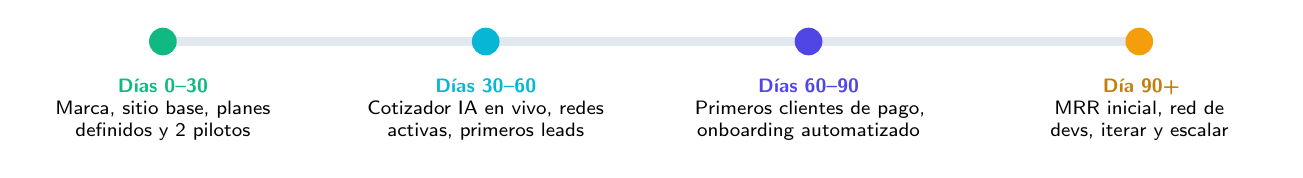
\begin{tikzpicture}
    % línea base
    \draw[wline,line width=3pt] (0,0) -- (12.4,0);
    \foreach \x/\c in {0/wmint,4.1/wcyan,8.2/wink,12.4/wamber}{\fill[\c] (\x,0) circle (5pt);}
    % hitos
    \node[anchor=north,text width=3.2cm,align=center,font=\scriptsize] at (0,-0.35)
      {\textbf{\color{wmint}Días 0–30}\\ Marca, sitio base, planes definidos y 2 pilotos};
    \node[anchor=north,text width=3.2cm,align=center,font=\scriptsize] at (4.1,-0.35)
      {\textbf{\color{wcyan}Días 30–60}\\ Cotizador IA en vivo, redes activas, primeros leads};
    \node[anchor=north,text width=3.2cm,align=center,font=\scriptsize] at (8.2,-0.35)
      {\textbf{\color{wink}Días 60–90}\\ Primeros clientes de pago, onboarding automatizado};
    \node[anchor=north,text width=3.2cm,align=center,font=\scriptsize] at (12.4,-0.35)
      {\textbf{\color{wamber!80!black}Día 90+}\\ MRR inicial, red de devs, iterar y escalar};
  \end{tikzpicture}}
  \end{center}
  \vspace{1.6cm}
  \begin{center}\footnotesize\color{wgray}
    \faFlagCheckered~ Meta a 90 días: cotizador en producción, presencia establecida y las primeras suscripciones activas.
  \end{center}
\end{frame}

%---------------------------------------------------------------- CIERRE ---
{\setbeamercolor{background canvas}{bg=wdark}
\begin{frame}[plain]
  
\begin{tikzpicture}[remember picture,overlay]
    \fill[wink,opacity=0.16] ([xshift=-2cm,yshift=2cm]current page.north east) circle (4.5cm);
    \fill[wcyan,opacity=0.10] ([xshift=1cm,yshift=-1cm]current page.south west) circle (3.5cm);
    \draw[wcyan,line width=6pt] ([xshift=1.4cm,yshift=1.5cm]current page.west) -- ++(0,-3cm);
    \node[anchor=west,align=left] at ([xshift=1.9cm,yshift=1.15cm]current page.west)
      {\color{white}\fontsize{30}{34}\selectfont\bfseries Ingeniería seria,\\ al alcance de cada PyME.};
    \node[anchor=west,align=left,text width=10cm] at ([xshift=1.92cm,yshift=-0.7cm]current page.west)
      {\color{wgray}\normalsize Un motor que automatiza del \textit{onboarding} al \textit{deploy}, un modelo de suscripción que alinea a todos, y dos mercados listos para empezar.};
    \node[anchor=west] at ([xshift=1.92cm,yshift=-1.9cm]current page.west)
      {\color{wcyan}\bfseries wodlie\,{\color{white}engine}\quad\color{wgray}\small · stifhlife@gmail.com · S4WLAND};
  \end{tikzpicture}
\end{frame}}

\end{document}
